\chapter{Light-Following Car}

%In our everyday life we see various insects that are attracted towards light. 

Light attracts life, or so they say! Be it sunflowers to seek life or angler fish to take it away, life does revolve around light. In this project, we will bring a little twist to the aforementioned dynamics by making an inanimate car follow light.

\subsection*{Components}
\begin{table}[H]
    \centering
    \begin{tabular}{|c|l|c|}\hline
     \textbf{\#} & \textbf{Components} &  \textbf{Amount}\\\hline
     1 & L298N: Motor driver       &  1\\\hline
     2 & LDR                        & 2\\\hline
     3 & 10 k$\Omega$ resistor      & 2 \\\hline
     4 & Push button                &  2\\\hline
     5 & 9V battery                 &  1\\\hline
     6 & 12V rechargeable battery   &  1\\\hline
     7 & Car chassis                & 1 \\\hline
     8 & Arduino UNO                & 1 \\\hline
     9 & Connecting wires           & - \\\hline
     
    \end{tabular}
\end{table}


\subsection*{Connections}

The circuit will need to be patched on the car. For this purpose, assemble the car chassis and connect the components as instructed below while fixing the components on the car at suitable positions on the chassis.

\begin{enumerate}[leftmargin=*] 
    \item Connect the 12 V power supply to the motor driver via a button. Also connect GND of Arduino with GND of the motor driver.
    \item Connect the 9V battery to Vin and GND pins of Arduino via a button. 
    \item Connect the control pins of the motor driver (IN1, IN2, IN3, IN4) to pins 6, 7, 8 and 9 of Arduino.
    \item Connect the output pins of the motor driver (OUT1, OUT2, OUT3, OUT4) with DC motors (fig. \ref{fig:bt-car}).
    \item Connect a 10k $\Omega$ resistor with one end of each LDR. 
    \item Connect the other end of the resistor to GND of Arduino. 
    \item Connect one end of both LDRs to GND of Arduino.
    \item Connect the junctions between the LDRs and the resisotrs with pin A0 and A1 of Arduino respectively.
\end{enumerate}

Fig. \ref{fig:lfc} illustrates the connections of the components.
	\begin{figure}[H]
	\centering 
	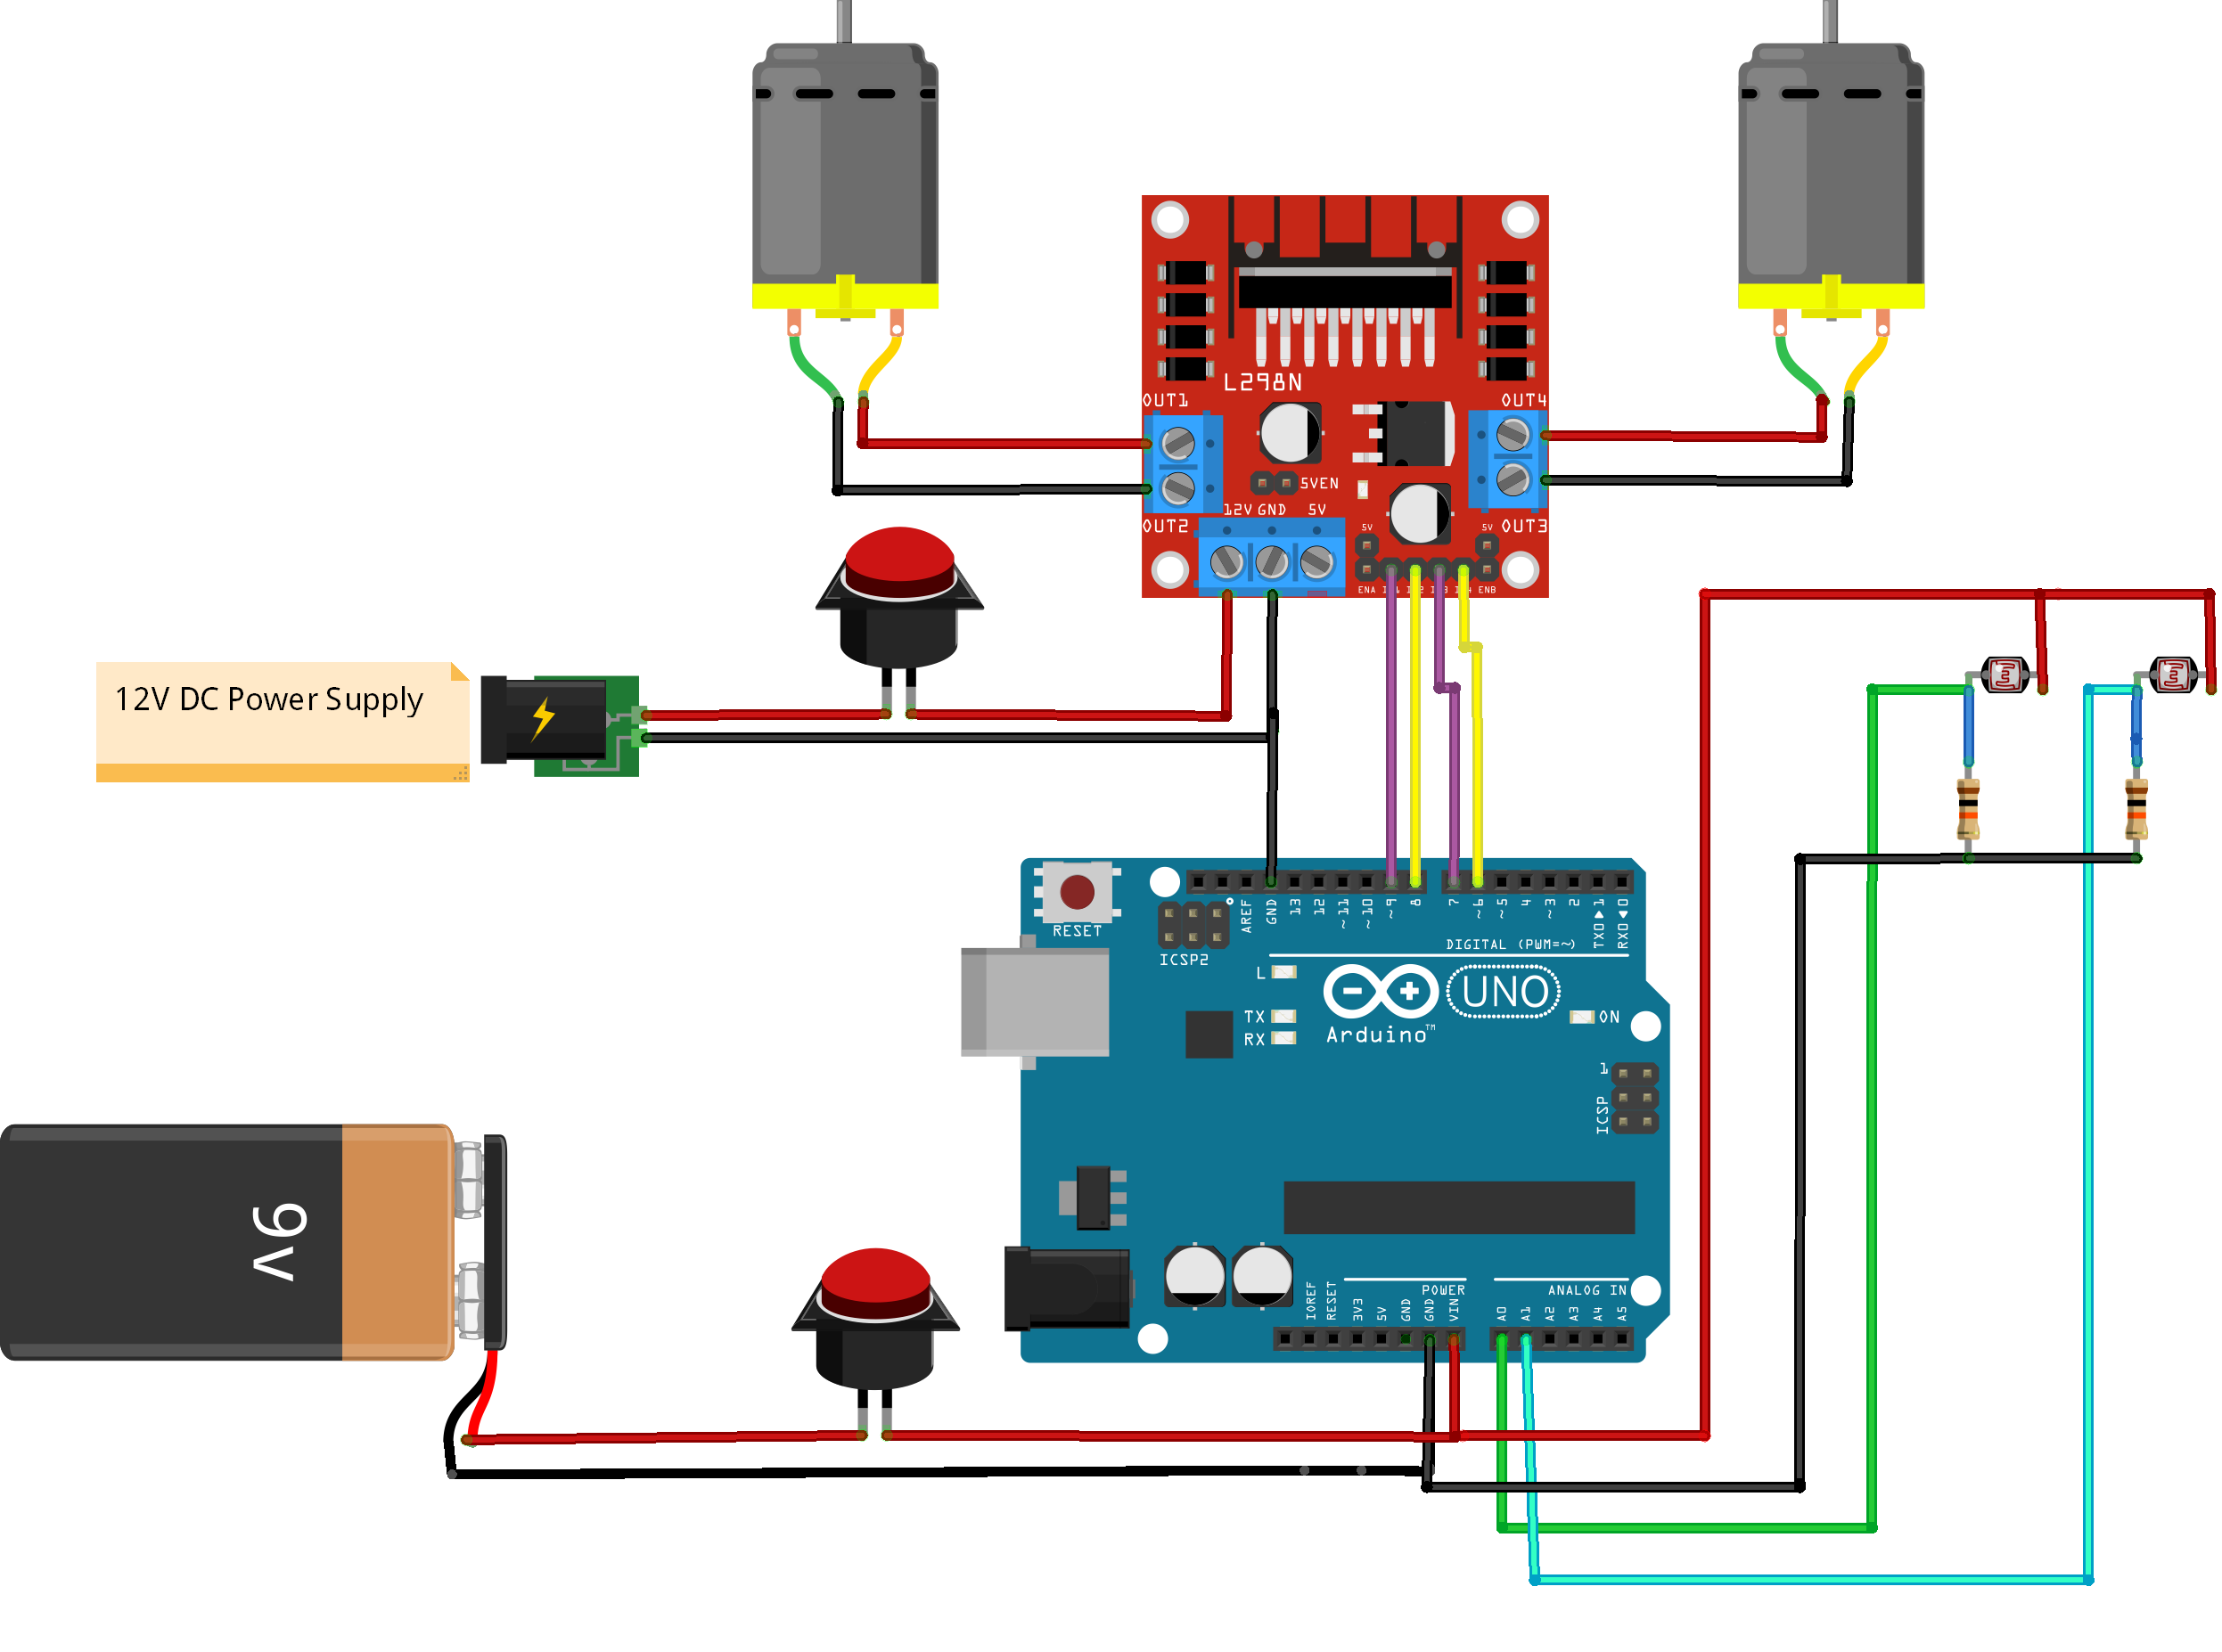
\includegraphics[width=0.6\linewidth]{recreational_exp/light following car_bb.png}
	\caption{Circuit diagram of Light Following Car}
	\label{fig:lfc}
	\end{figure}
	
\subsection*{Procedure}
\begin{enumerate}[leftmargin=*]
    \item Copy lst.\ref{list:light-car} to a new Arduino sketchbook. Upload the code to your Arduino board.
    \item Open flashlight of your mobile and shine it on one of the LDR and observe direction of the movement of car. It will follow the light. 
\end{enumerate}

\begin{lstlisting}[language=Arduino, numbers=none, caption={Code for light-following car}, captionpos=b, label={list:light-car}]
// motor 1 pins 
int m11=8;
int m12=9;

// motor 2 pins
int m21=6;
int m22=7;

//speed of motors 
int spd = 255;

//Pims of LDR
int LDR1 = A0;
int LDR2 = A1;

// variables to red value from LDRs
int LDRleft; 
int LDRright;
int tolerence = 20 ; // set this value according to environment 

// Defining functions
void forward(int dum){
  analogWrite(m11, dum);
  analogWrite(m12, LOW);
  analogWrite(m21, dum);
  analogWrite(m22, LOW);
}
void right(int dum){
  analogWrite(m11, dum);
  analogWrite(m12, LOW);
  analogWrite(m21, LOW);
  analogWrite(m22, dum);
}
void left(int dum){
  analogWrite(m11, LOW);
  analogWrite(m12, dum);
  analogWrite(m21, dum);
  analogWrite(m22, LOW);
}
void stay (void){
  analogWrite(m11, LOW);
  analogWrite(m12, LOW);
  analogWrite(m21, LOW);
  analogWrite(m22, LOW);
}

void setup() {
      // put your setup code here, to run once:
    Serial.begin(9600);
    pinMode(m11, OUTPUT);
    pinMode(m12, OUTPUT);
    pinMode(m21, OUTPUT);
    pinMode(m22, OUTPUT);
}

void loop() {
   LDRleft = analogRead(LDR1); 
   LDRright = analogRead(LDR2);
    
   if(((LDRleft - LDRright) < tolerence) and  ((LDRleft - LDRright) >= 0) ){
      forward(spd);
    }
   else if(((LDRright - LDRleft) < tolerence) and  ((LDRright - LDRleft) >= 0) ){
      forward(spd);
    }
    else if((LDRleft - LDRright) >=  tolerence){
      left(spd);
    }
    else if((LDRright - LDRleft) >=  tolerence){
      right(spd);
    }
    else{
      stay();
    }
}
\end{lstlisting}

\subsection*{Precautions}
\begin{itemize}[leftmargin=*]
    \item Change the threshold value in the code according to the brightness of environment.
    \item If the car is not moving according to the transmitted commands, try swapping the control pins of the motor driver.
\end{itemize}